
\documentclass{beamer}
\usetheme{Electromagnetism}
\usepackage{Electromagnetism}
\graphicspath{{pictures/}}
% -------------------------------------- Grid
%-------------------------------------------------------
\makeatletter
\def\grd@save@target#1{%
  \def\grd@target{#1}}
\def\grd@save@start#1{%
  \def\grd@start{#1}}
\tikzset{
  grid with coordinates/.style={
    to path={%
      \pgfextra{%
        \edef\grd@@target{(\tikztotarget)}%
        \tikz@scan@one@point\grd@save@target\grd@@target\relax
        \edef\grd@@start{(\tikztostart)}%
        \tikz@scan@one@point\grd@save@start\grd@@start\relax
        \draw[minor help lines] (\tikztostart) grid (\tikztotarget);
        \draw[major help lines] (\tikztostart) grid (\tikztotarget);
        \grd@start
        \pgfmathsetmacro{\grd@xa}{\the\pgf@x/1cm}
        \pgfmathsetmacro{\grd@ya}{\the\pgf@y/1cm}
        \grd@target
        \pgfmathsetmacro{\grd@xb}{\the\pgf@x/1cm}
        \pgfmathsetmacro{\grd@yb}{\the\pgf@y/1cm}
        \pgfmathsetmacro{\grd@xc}{\grd@xa + \pgfkeysvalueof{/tikz/grid with coordinates/major step}}
        \pgfmathsetmacro{\grd@yc}{\grd@ya + \pgfkeysvalueof{/tikz/grid with coordinates/major step}}
        \foreach \x in {\grd@xa,\grd@xc,...,\grd@xb}
        \node[anchor=north] at (\x,\grd@ya) {\pgfmathprintnumber{\x}};
        \foreach \y in {\grd@ya,\grd@yc,...,\grd@yb}
        \node[anchor=east] at (\grd@xa,\y) {\pgfmathprintnumber{\y}};
      }
    }
  },
  minor help lines/.style={
    help lines,
    step=\pgfkeysvalueof{/tikz/grid with coordinates/minor step}
  },
  major help lines/.style={
    help lines,
    line width= 0.5pt,
    step=\pgfkeysvalueof{/tikz/grid with coordinates/major step}
  },
  grid with coordinates/.cd,
  minor step/.initial=.2,
  major step/.initial=1,
  major line width/.initial=2pt,
}
\makeatother
\usepackage{cancel}
\begin{document}

% ============================== Слайд ## ===================================
\begin{frame}{Як заряджають тіла?}{Трибоелектричний ефект}
	\tikz[remember picture,overlay] \node[opacity=0.7,inner sep=0pt,
		anchor=south east] at (current page.south
	east){
\includegraphics[width=3cm]{Tribocat}};

	\tikz[remember picture,overlay] \node[opacity=0.7,inner sep=0pt,
		anchor=north west] at ([yshift=-1.5cm]current page.north
	west){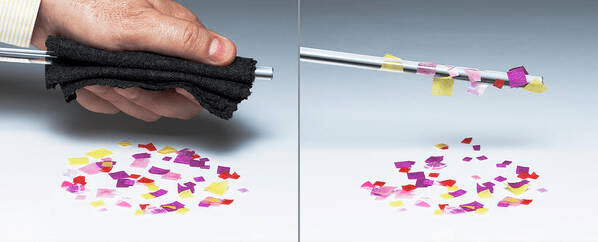
\includegraphics[width=5cm]{charging-by-friction}};

	\tikz[remember picture,overlay] \node[opacity=0.7,inner sep=0pt,
		anchor=north east] at ([yshift=-1.7cm]current page.north
	east){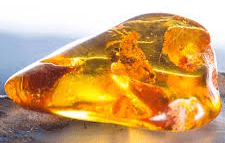
\includegraphics[width=3cm]{Amber}};

	\begin{onlyenv}<1>
		\begin{block}{}
			\alert{Трибоелектричний ефект} --- поява електричних зарядів у
			матеріалі через тертя.
		\end{block}

		\begin{block}{}\justifying
			Деякі матеріали стають електрично зарядженими після того, як вони
			входять у
			фрикційний контакт з іншим матеріалом.
		\end{block}

		\begin{exampleblock}\justifying\small
			Слово <<\alert{електрика}>> походить від грецького
			<<$\eta\lambda\varepsilon\kappa\tau\rho o \nu$>>
			(\alert{електрон}), що означає <<\alert{бурштин}>>. Люди помітили,
			що бурштин, натертий об хутро, притягує дрібні предмети, і це
			явище згодом стало основою для дослідження електричних явищ.
		\end{exampleblock}
	\end{onlyenv}

	\begin{onlyenv}<2>
        \vspace*{2em}
		\begin{block}{}\justifying
			Матеріали, що виявляють трибоелектричний ефект, прийнято
			розташовувати в \alert{трибоелектричний ряд}, один кінець якого є
			позитивним, а інший --- негативним. Під час тертя пари матеріалів
			з ряду, матеріал, розташований ближче до позитивного кінця ряду,
			зарядиться позитивно, а інший --- негативно.
		\end{block}
		\begin{center}
			\begin{tikzpicture}[scale=0.5, transform shape]
				% Градієнт фону
				\shade[left color=blue!30, right color=red!30] (-5.5, -.5) rectangle (5.5, -3.5);

				\node[single  arrow, single  arrow head extend=.5cm, left color=blue!50, right color=red!50, text=white, font={\bf \large}, inner sep=0.3cm]
				(doublearrow)
				{--\hspace*{10.5cm}+};

				% Трибоелектричний ряд
				\node[align=center, rotate=90] at (5,  -2) {Хутро};
				\node[align=center, rotate=90] at (4,  -2) {Фланель};
				\node[align=center, rotate=90, align=center, text width=2.5cm] at (3,  -2) {Слонова\\ кістка};
				\node[align=center, rotate=90] at (2,  -2) {Пір'я};
				\node[align=center, rotate=90] at (1,  -2) {Флінтглас};
				\node[align=center, rotate=90] at (0,  -2) {Шовк};
				\node[align=center, rotate=90] at (-1, -2) {Алюміній};
				\node[align=center, rotate=90] at (-2, -2) {Поліестер};
				\node[align=center, rotate=90] at (-3, -2) {Папір};
				\node[align=center, rotate=90] at (-4, -2) {Бурштин};
				\node[align=center, rotate=90] at (-5, -2) {Ебоніт};
			\end{tikzpicture}
		\end{center}
	\end{onlyenv}
\end{frame}

\end{document}